\documentclass[12pt]{article}
\usepackage[utf8]{inputenc}
\usepackage[english]{babel}
\usepackage[letterpaper, portrait, margin=1in]{geometry}
\usepackage{amsmath}
\numberwithin{equation}{section}
\usepackage{amssymb}
\usepackage{graphicx}
\usepackage{wrapfig}
\usepackage{parskip}
\usepackage{xcolor}
\usepackage{physics}
\usepackage{empheq}
\usepackage{cancel}
\usepackage{hyperref}
\hypersetup{colorlinks = true, urlcolor = blue, linkcolor = red, citecolor = red}
\usepackage{enumerate}
\usepackage{tikz}
\usepackage{float}
\usepackage{tcolorbox}
\usepackage{booktabs}

\author{Yi J Zhu}
\title{Density of States}
\date{\today}

\begin{document}

\maketitle

\subsection{Density of States}
It is often useful to know the density of states (DOS) as function of energy. To begin, how is the DOS defined?

First, we define $N(\epsilon)$ as the total number of states with energy less than or equal to $\epsilon$. Then, the density of states is,
\begin{equation}
    D(\epsilon) = \dv{N}{\epsilon}
\end{equation}
In other words,
\begin{equation}
    N(\epsilon) = \int_0^\epsilon D(\epsilon')\dd{\epsilon'}
\end{equation}

\subsection{Particle in a Box}

The energy eigenstates of a particle in a cubical box of length $L$ with no potential ($V=0$) are,

\begin{equation}
    \psi(x,y,z) = \sin\left(\frac{n_x\pi}{L}x\right)\sin\left(\frac{n_y\pi}{L}y\right)\sin\left(\frac{n_z\pi}{L}z\right)
\end{equation}
where,
\begin{equation}
    \epsilon = \frac{\pi^2\hbar^2}{2mL^2}(n_x^2 + n_y^2 + n_z^2); \quad n_x, n_y, n_z \in \mathbb{N}
\end{equation}

The states are equal spaced in three-dimensions in ``n-space," but how do we relate this to energy? If we define the variable,
\begin{equation}
    n = \sqrt{n_x^2 + n_y^2 + n_z^2}
    \label{eq:n}
\end{equation}
then,
\begin{equation}
    \epsilon = \frac{\pi^2\hbar^2}{2mL^2} n^2
\end{equation}
Now, we must find $N(n)$. Notice that the contour of $n$ is a sphere in ``n-space." However, $n_x,n_y,n_z>0$, so $N(n)$ must be the volume of a octant of radius $n$.

\begin{figure}[h!]
  \begin{center}
    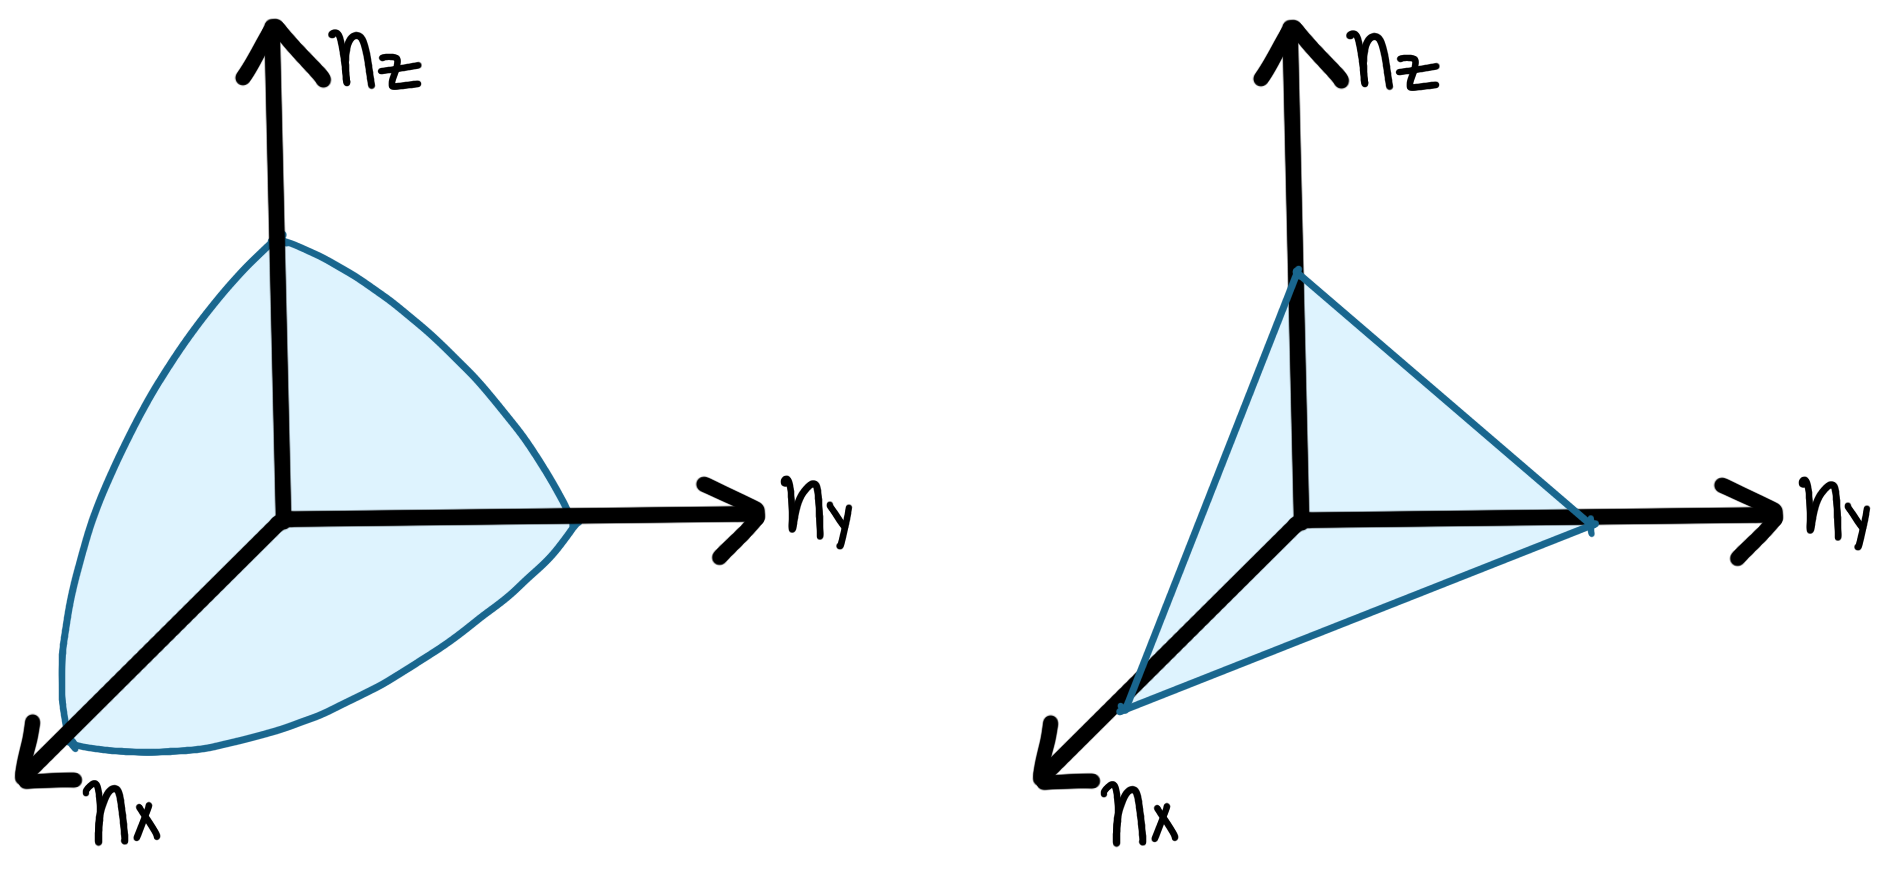
\includegraphics[width=0.6\textwidth]{contour}
  \end{center}
  \caption{(a) contour for $n=\sqrt{n_x^2 + n_y^2 + n_z^2}$, (b) contour for $n=n_x+n_y+n_z$}
  \label{fig:contour}
\end{figure}

Therefore, the number of states up to $n$ is given by,
\begin{equation}
    N(n) = \frac{1}{8}\left(\frac{4}{3}\pi n^3\right) = \frac{\pi}{6}n^3
    \label{eq:N}
\end{equation}
The density of states as a function of $n$,
\begin{equation}
    D(n) = \dv{N}{n} = \frac{\pi}{2}n^2
\end{equation}
Finally,
\begin{equation}
    D(n)\dd{n} = D(\epsilon)\dd{\epsilon}
\end{equation}
\begin{equation}
    D(\epsilon) = D(n) \left(\dv{n}{\epsilon}\right) = \left(\frac{\pi}{2}n^2\right)\left(\frac{mL^2}{\pi^2\hbar^2 n}\right) = \frac{mL^2}{2\pi\hbar^2}n
\end{equation}
Where $n$ is a function of $\epsilon$,
\begin{equation}
    D(\epsilon) = \frac{mL^2}{2\pi\hbar^2} \sqrt{\frac{2mL^2\epsilon}{\pi^2\hbar^2}}
\end{equation}
\begin{equation}
    \boxed{D(\epsilon) = \frac{L^3}{2\pi^2}\left(\frac{2m}{\hbar^2}\right)^{3/2}\epsilon^{1/2}}
\end{equation}
This method generalizes to 1 and 2-dimensions.

\subsection{Harmonic Oscillator}
Suppose now that we are trying to find the DOS of a harmonic oscillator with energy (ignoring the zero-point energy),
\begin{equation}
    \epsilon = (n_x+n_y+n_z)\hbar\omega
\end{equation}
Now, the energy is no longer a function of $n$ as we have defined it in the previous section (eq. \ref{eq:n}). We must now define $n$ to be,
\begin{equation}
    n = n_x + n_y + n_z
\end{equation}
\begin{equation}
    \epsilon = n\hbar\omega
\end{equation}

Again, we can find $N(n)$; but now, notice that the contour of $n$ is no longer a sphere, but a plane (Fig. \ref{fig:contour}). Thus,
\begin{equation}
    N(n) = \frac{1}{3}A\cdot h = \frac{1}{3}\left(\frac{1}{2}n^2\right)\cdot n = \frac{n^3}{6}
\end{equation}
As before, we can manipulate this into the DOS in energy,
\begin{equation}
    D(n) = \dv{N}{n} = \frac{n^2}{2}
\end{equation}
\begin{equation}
    D(\epsilon) = D(n) \left(\dv{n}{\epsilon}\right) = \left(\frac{n^2}{2}\right)\left(\frac{1}{\hbar\omega}\right) 
\end{equation}
\begin{equation}
    \boxed{D(\epsilon) = \frac{\epsilon^2}{2(\hbar\omega)^3}}
\end{equation}

\end{document}
